
\section{Resultados}

\subsection{Linked Communities}
En esta sección procedemos a obtener las comunidades existentes dentro de nuestra red de proteínas, obtenida en la sección anterior.

Antes debemos tener claro que las comunidades son conjuntos de nodos relacionados entre sí que poseen funciones semejantes y que buscan conseguir un objetivo común. Es por ello por lo que la identificación de las comunidades es un problema relevante para muchas áreas de investigación como la sociología, la biología o la informática.

En general, la comunidades se pueden clasificar en dos tipos, las que están formadas por nodos y las que están formadas por enlaces.

\begin{itemize}
\item Comunidad de nodos: Se tratan de subgrafos formados por nodos densamente conectados entre ellos, pero muy poco conectados con los nodos de alrededor, como se muestra en la imagen. 


\begin{center}

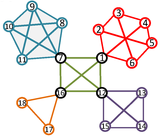
\includegraphics[width=70mm,scale=1.2]{report/figures/nodes.png}

\caption{\textit{Comunidad de nodos}}

\end{center}


\item Link community: Consiste en un subgrafo en el que existe una gran cantidad de enlaces pero muy pocos con las comunidades externas. La forma de detectar estos conjuntos es mediante la división de los enlaces de la red. En estas particiones, las conexiones determinan una comunidad, pero los nodos pueden pertenecer a varias comunidades. 


\begin{center}
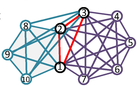
\includegraphics[width=70mm,scale=1.2]{report/figures/links.png}


\caption{\textit{Link community}}

\end{center}

Con esto queremos remarcar que la importancia de la detección de estos subgrafos se debe a que en el campo de la biología, permiten encontrar módulos proteicos con una misma función celular o predecir las funciones de las proteínas.

Por tanto, diseñaremos un código en R que nos permite la detección de las comunidades con el fin de filtrar aquellas que son más importantes (centralidad). De esta forma, podemos llevar a cabo un enriquecimiento funcional de las mismas y así obtener algunas de las funciones celulares que determinan red del SARS-CoV-2.

Además, en el código siguiente se incluyen diferentes gráficas para la visualización de las comunidades.
\end{itemize}

A lo largo de la ejecución del código hemos añadido distintas gráficas para la representación de las comunidades. A continuación se muestra un dendograma de las \textit{link communities}, en el que se puede apreciar una gran cantidad de comunidades. En esta imagen es difícil ver la centralidad de las comunidades, por lo que haremos más representaciones.

\begin{lstlisting}
#link communities dendogram
png(file="linkcomm_dend.png")
plot(proteins.mapped.network.lc, type = "dend")
dev.off()
\end{lstlisting}

\begin{center}
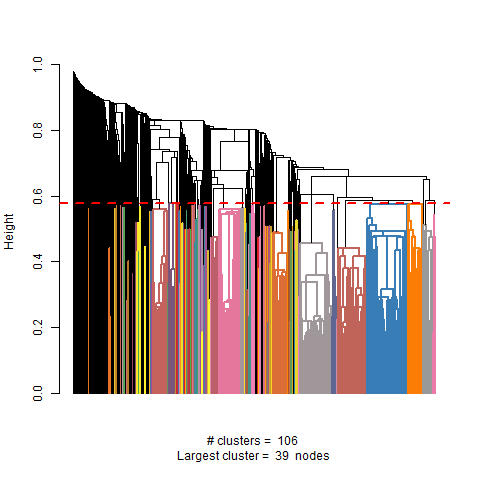
\includegraphics[width=90mm,scale=1]{report/figures/linkcomm_dend.png}


\caption{\textit{Dendograma de Linked Communities}}

\end{center}


Empleando el diseño \textbf{ Fruchterman Reingold} se puede obtener una visión más amplia de las comunidades. 

\begin{lstlisting}
#link communities Fruchterman Reingold layout
png(file="linkcomm_layout.fruchterman.reingold.png")
plot(proteins.mapped.network.lc, type = "graph", layout =
layout.fruchterman.reingold, vlabel=FALSE)
dev.off()
\end{lstlisting}

\begin{center}

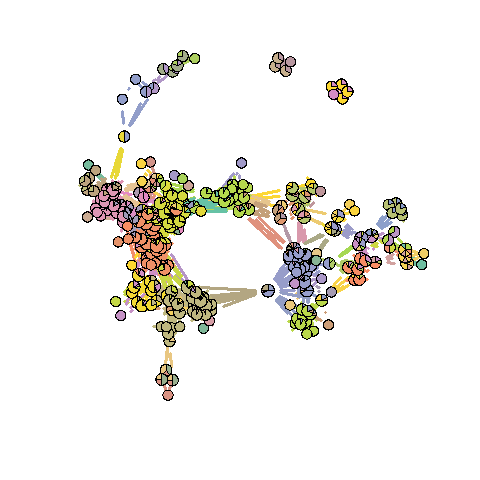
\includegraphics[width=90mm,scale=1]{report/figures/linkcomm_layout.fruchterman.reingold.png}


\caption{\textit{Linked Communities con Fruchterman Reingold layout }}

\end{center}

Sin embargo, lo que nos interesa en este caso es obtener la \textbf{'centralidad comunitaria'} pues se define como la suma de las áreas con mayor influencia sobre los nodos vecinos de la red. Por tanto, nos permite obtener aquellos clusters que ejercen una mayor influencia sobre la red, pudiendo ser determinantes en la funcionalidad de la misma.

Por otra parte, la \textbf{modularidad} consiste en el grado de separación y recombinación existente entre los componentes de una red. Es decir, se considera como una medida de la presencia de estructura comunitaria. Esto permite la búsqueda de comunidades, quedándonos con aquellas que tengan un valor de modularidad positivo y lo más grande posible (modularidad optimizada).

Por ello, hemos calculado la modularidad de las comunidades de nuestra red y hemos representado el valor de la modularidad para cada una de ellas.

\begin{lstlisting}
# Community centrality
community.centrality <- getCommunityCentrality(proteins.mapped.network.lc)

#modularity of the communities
community.connectedness <- getCommunityConnectedness(
proteins.mapped.network.lc,conn = "modularity") 

png(file="communities_modularity.png")
plot(proteins.mapped.network.lc, type = "commsumm", summary = "modularity")
dev.off()
\end{lstlisting}
\begin{center}
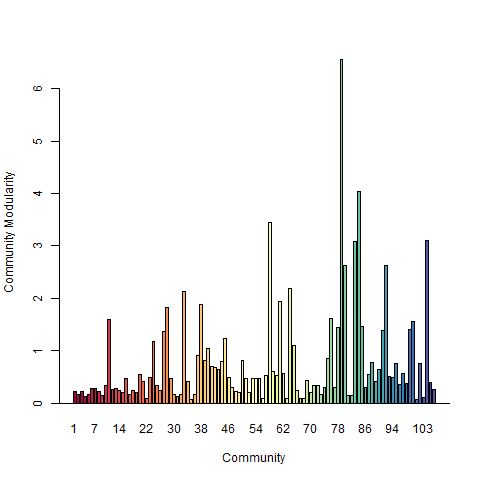
\includegraphics[width=90mm,scale=1]{report/figures/communities_modularity.png}

\caption{\textit{Diagrama de barras de la modularidad de las comunidades}}

\end{center}
En la imagen se observa claramente como hay una comunidad con una modularidad muy alta, lo que indica que esta es más influyente en la red que el resto, concretamente la comunidad 79.


\begin{lstlisting}
# Focus on one linkcomm
#plot one cluster with maximun community modularity
png(file="cluster12_graph.png")
plot(proteins.mapped.network.lc, type = "graph", clusterids =
community.connectedness.maximum, vlabel=FALSE)
dev.off()

\end{lstlisting}

\begin{center}
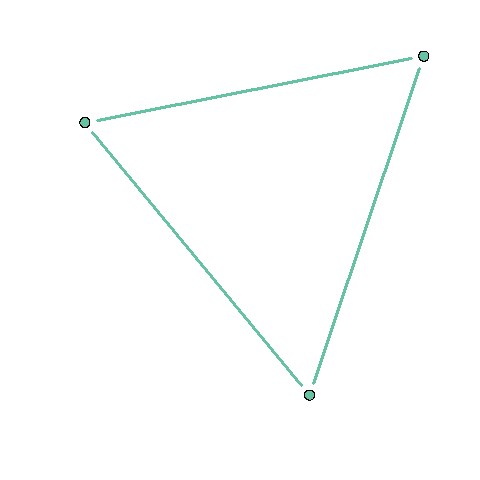
\includegraphics[width=70mm,scale=1]{report/figures/cluster_graph.png}
\end{center}

Por tanto, realizaremos un análisis funcional centrándonos en aquellas comunidades con una modularidad mayor, para determinar si sus funciones moleculares son determinantes o no.
